\section{LibrePCB Fab}

\begin{frame}{\secname}

  The easiest and fastest way to order a PCB!

  \begin{tikzpicture}
    \node (img1)
    {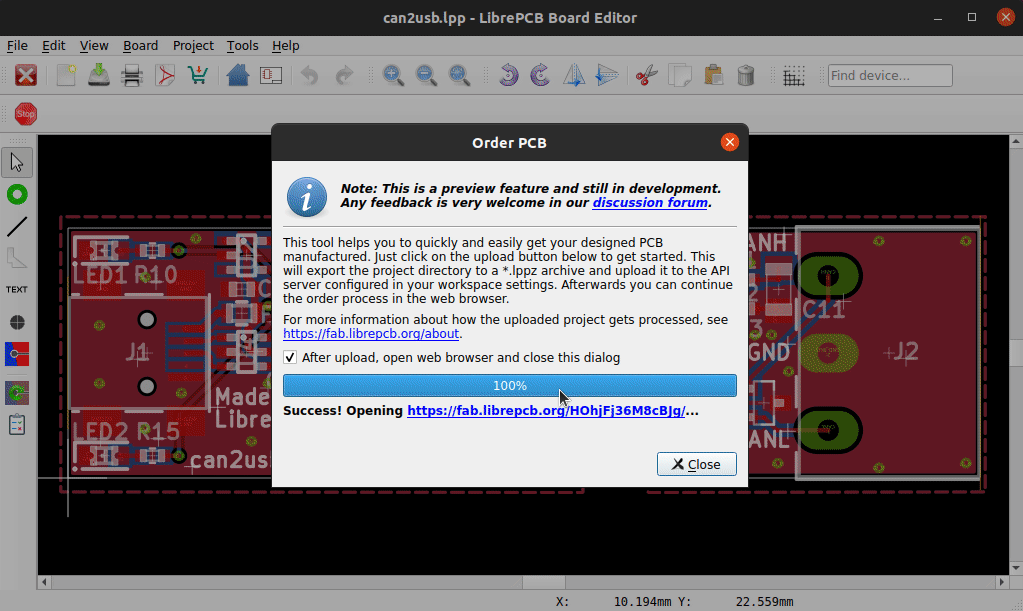
\includegraphics[width=7cm]{images/order_pcb_1.png}};
  \end{tikzpicture}

\end{frame}

\note{
  The last feature I want to mention is a completely new way to start
  ordering the PCB.\\

  Generating Gerber and Excellon files is still a challenge, especially for
  beginners. It's not easy to understand how to generate correct production
  data files, especially since every PCB manufacturer has slightly different
  requirements on the production data format. For example regarding file
  naming, file extension, Gerber format version, merged or split drill files,
  there are a lot of things you can do the wrong way.\\

  Therefore we integrated a much simpler way to order the PCB
  directly from within the application. A shopping cart symbol in the
  application opens a dialog which quickly explains how the feature works.
}

\begin{frame}[noframenumbering]{\secname}

  The easiest and fastest way to order a PCB!

  \begin{tikzpicture}
    \node (img1)
    {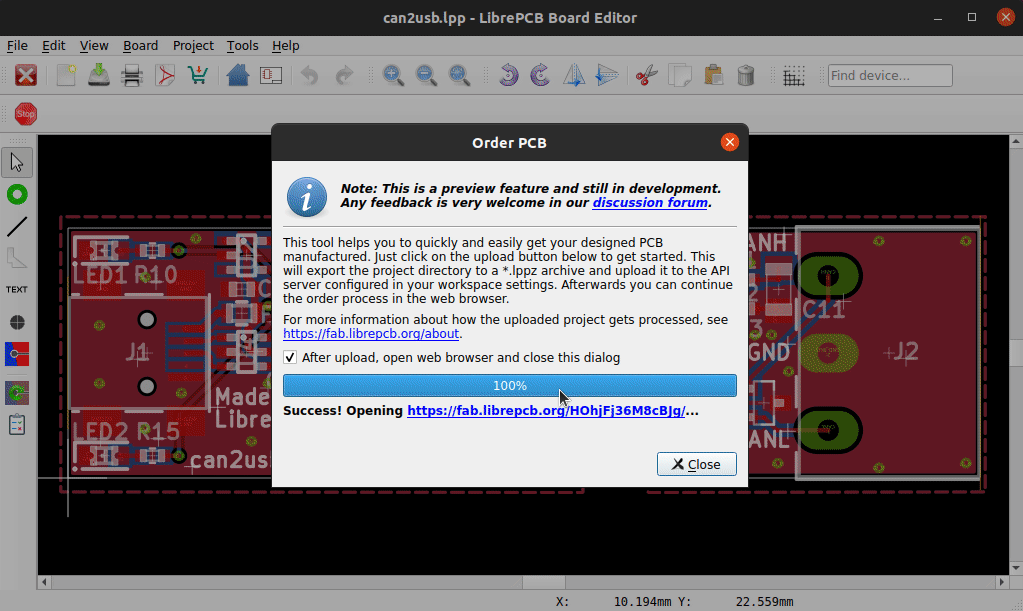
\includegraphics[width=7cm]{images/order_pcb_1.png}};

    \node (img2) [xshift=3.3cm,yshift=-1cm]
    {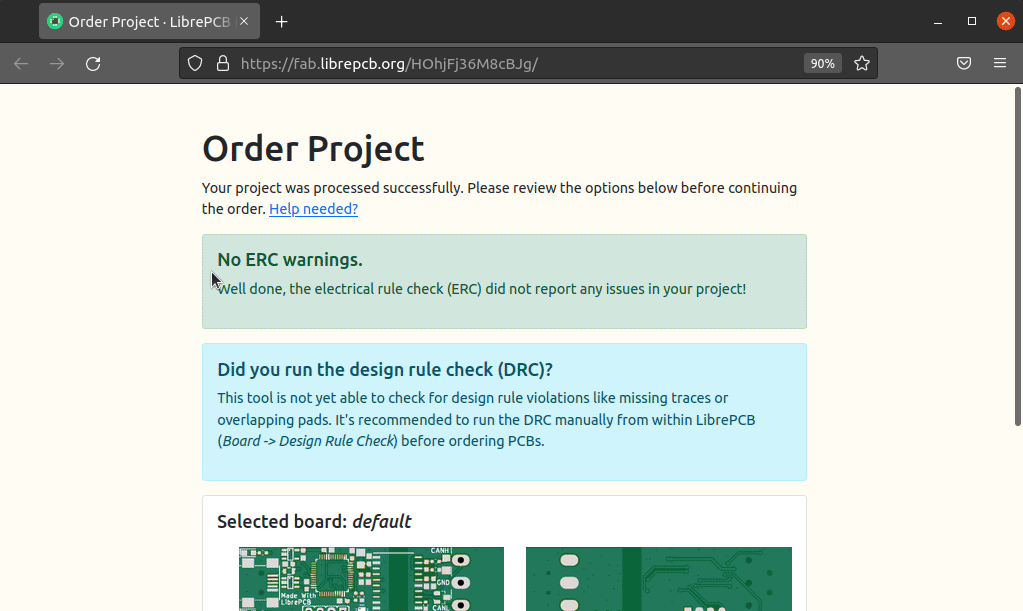
\includegraphics[width=7cm]{images/order_pcb_2.png}};
  \end{tikzpicture}

\end{frame}

\note{
  With a simple button click, the PCB
  is opened in the web browser, and with another button click you are forwarded
  to the Aisler website, where you now can see the price and complete the
  order.
}

\begin{frame}[noframenumbering]{\secname}

  The easiest and fastest way to order a PCB!

  \begin{tikzpicture}
    \node (img1)
    {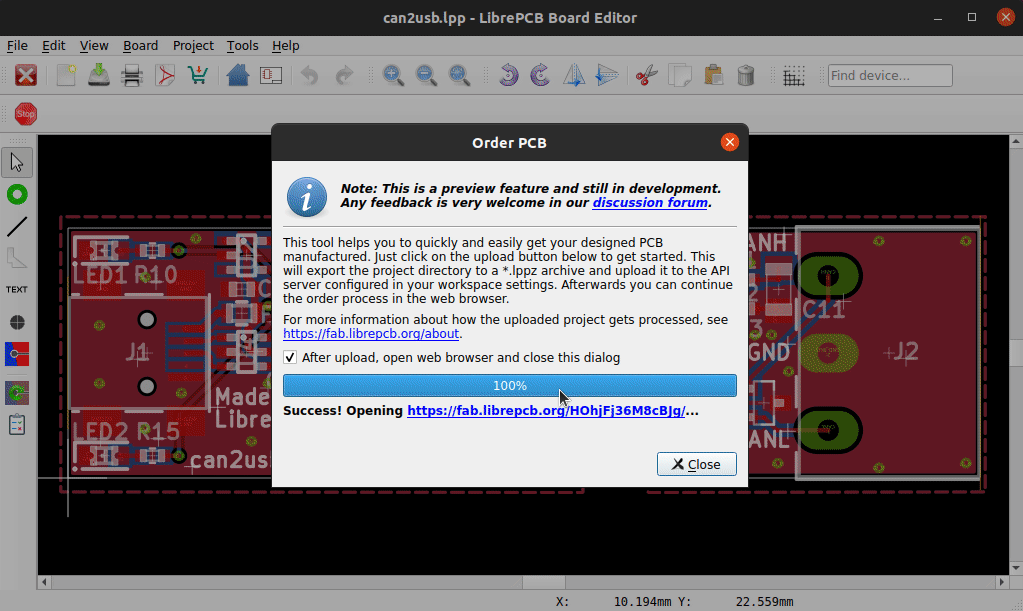
\includegraphics[width=7cm]{images/order_pcb_1.png}};

    \node (img2) [xshift=3.3cm,yshift=-1cm]
    {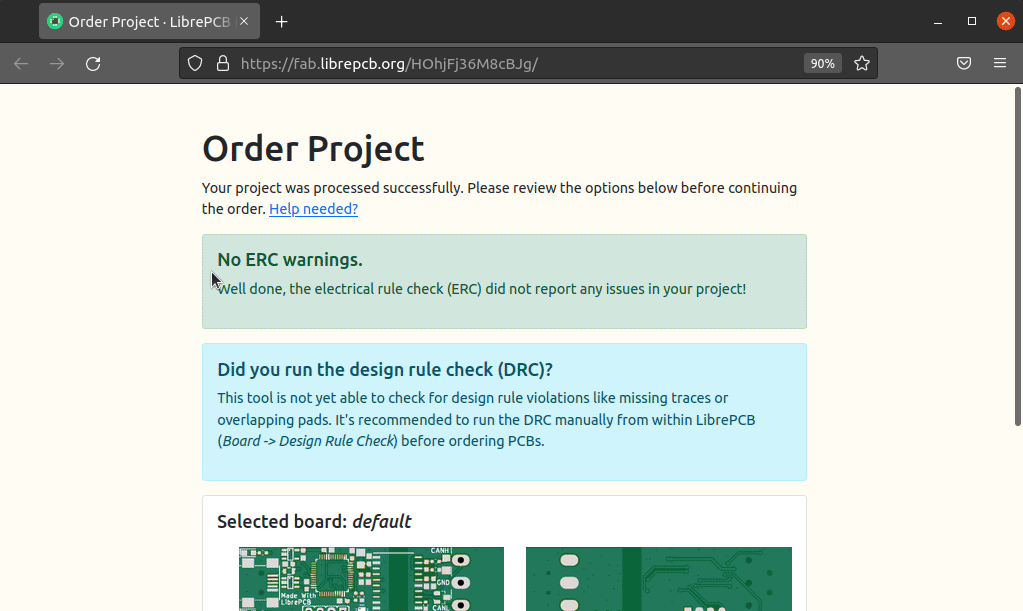
\includegraphics[width=7cm]{images/order_pcb_2.png}};

    \node (img3) [xshift=6.6cm,yshift=-2cm]
    {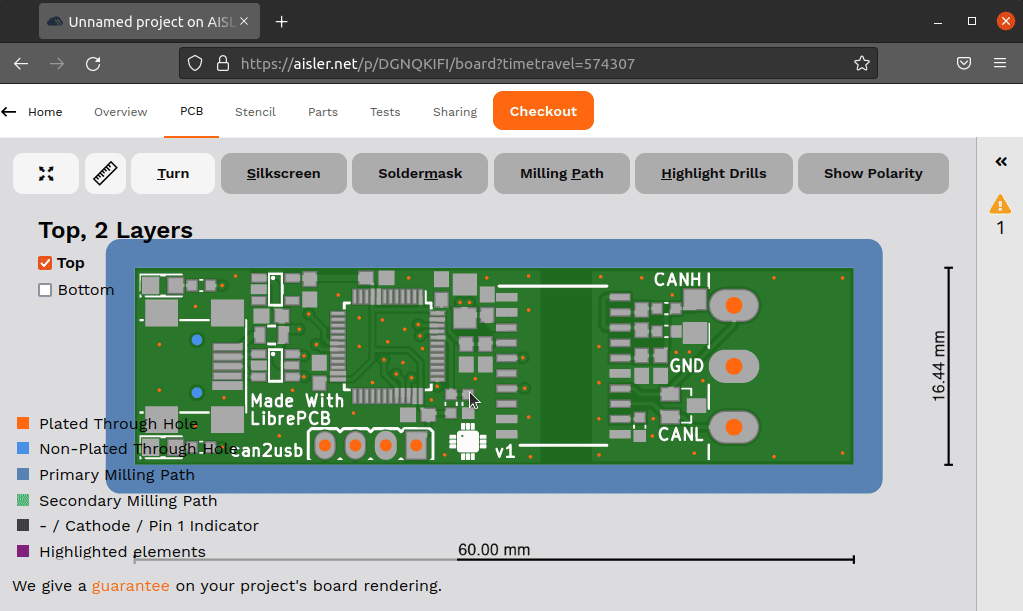
\includegraphics[width=7cm]{images/order_pcb_3.png}};
  \end{tikzpicture}

\end{frame}

\note{
  With a simple button click, the PCB
  is opened in the web browser, and with another button click you are forwarded
  to the Aisler website, where you now can see the price and complete the
  order.

  Let's quickly demonstrate how this works.\\

  Many thanks to Aisler who does not only provide an API for this service,
  but even makes a donation to LibrePCB for every order made
  with this feature. So actually using this feature is not only an easy
  and fast way to order the PCB, but also to support the LibrePCB project!
}
